\section{Indledning}

\myworries{Formål og mål med projektet.}\\

% ------------------------ Baggrund for projektet ------------------------------------------------
Når et program bliver broadcasted på en TV station skal krediteringer vises. Dette gøres i slutningen af programmet, i maksimalt 30 sekunder. Det betyder, at der ikke altid er tid til at vise alle krediteringer, og derfor prioriteres de før de vises. \\
Hvis de 30 sekunder for hvert program kunne frigøres, kan danske TV stationer bruge tiden på at vise noget andet, som f.eks. reklamer og promovering af eget indhold. Derved har TV 2 mulighed for at øge deres årlige indtægter med op til 60 millioner kroner. \\
TV 2 har brug for et system, der kan administrere krediteringer for programmer produceret i Danmark. Hertil skal der kunne tilføjes nye krediteringer i systemet for nye produktioner, samt det skal være muligt at kunne søge efter eksisterende krediteringer. Det skal være muligt at kunne se hvilken rolle en given person har haft i en produktion, da denne person kan have haft flere forskellige roller på flere forskellige produktioner.

% ------------------------ Projektets rammer og baggrunden for projektet -------------------------
\subsection{Projektrammer}
Denne sektion har til formål at opridse rammerne for projektet, samt hvilket område projektgruppen arbejder indenfor.

\subsubsection{Krav til Projektet}
Systemet skal så vidt muligt skrives i programmeringssproget Java. \\
Krediterings-data skal lagres i en database, og i dette projekt skal den brugte database være SQL baseret. Der skal bruges PostgreSQL.\\
Systemet forventes ikke at være et færdigt system, men en række forslag til løsninger der opfylder systembehovet. Forslagene skal inkludere:

% ------------------------- OPDATER DENNE TIDSPLAN ----------------------------------------------
\begin{itemize}
    \item Krav
    \item Analyse
    \item Design
    \item Implementering
    \item Test
\end{itemize}
% ----------------------------------------------------------------------------------------------

\noindent
Producere der kan tilføje og redigere i krediteringerne, skal kun have mulighed for at redigere i de produktioner, de selv ejer.\\
Det forventes at krediteringssystemet er kompatibelt med andre systemer (f.eks. fra Stofa, YouSee etc.).

\subsubsection{Tidsplan}
Tidsplanen har til formål at skabe overblik og styring over projektet. 
Den giver gruppemedlemmerne et overblik over, hvornår de forskellige dele af projektet skal starte og slutte, og derved bliver det hurtigt klart hvis tidsplanen skrider. \\

\begin{landscape}
    \begin{figure}
        \centering
        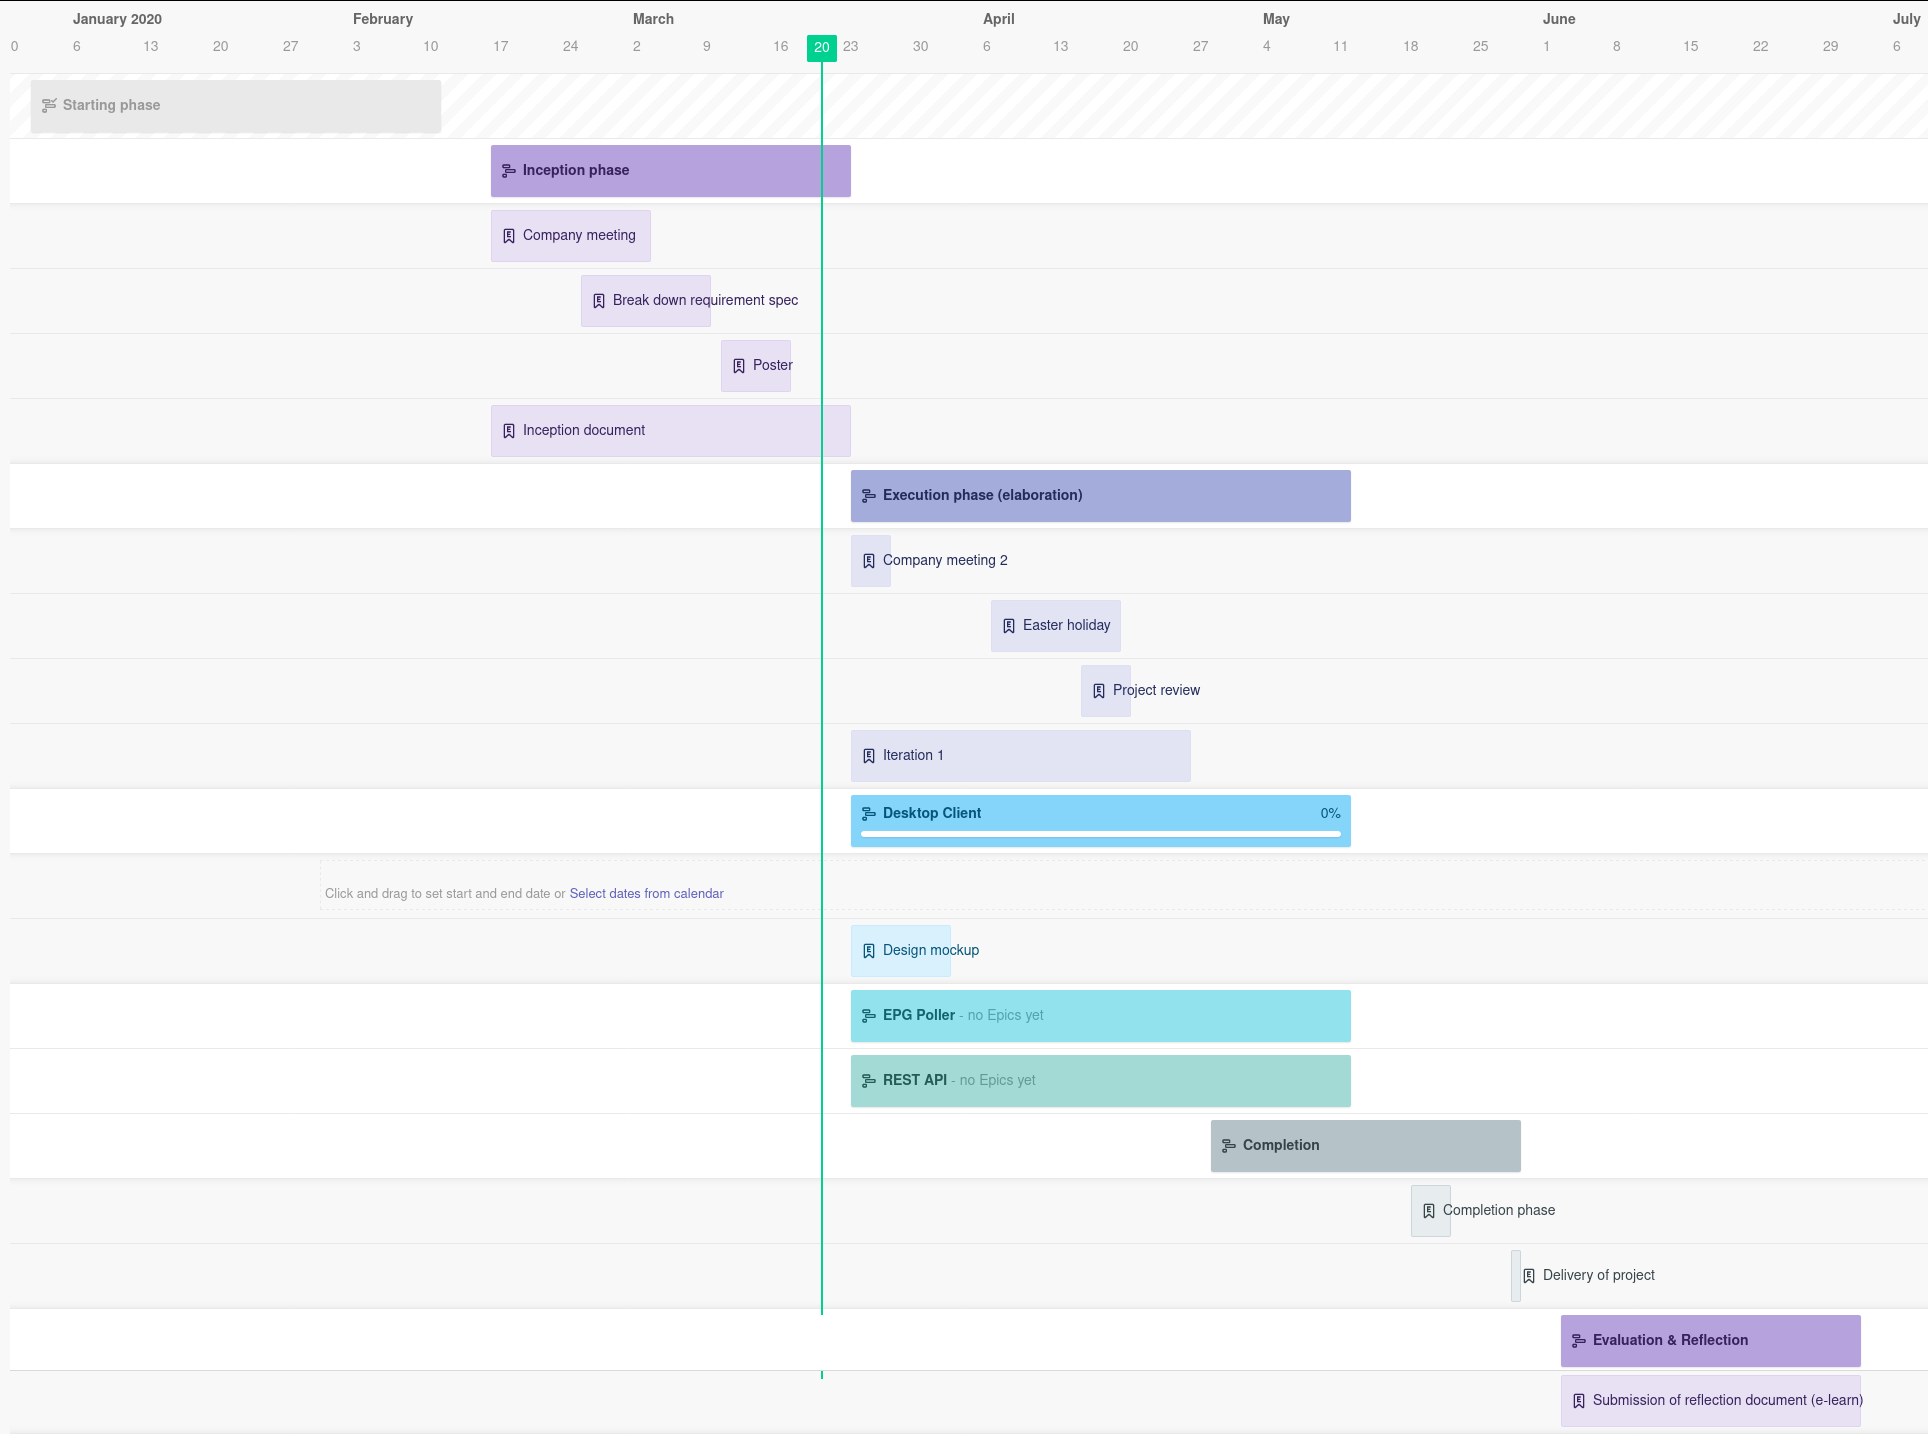
\includegraphics[scale=0.30]{figures/grantt_udvidet.png}
        \caption{Tidsplan for projektet}
        \label{fig:gantt}
    \end{figure}{}
\end{landscape}


% ------------------------ Resume af udleverede case ----------------------------------------------
\subsubsection{Igangsættende Problem}
TV2 ønsker at frigøre 30 sekunders krediterings tekster efter hvert program, så de i stedet kan bruge tiden på at vise reklamer. Problemet består i at disse krediterings tekster, så skal vises på en anden platform. I tabel \ref{table:kravFraCase} ses kravene fra TV2's projektcase: \\

\begin{table}[ht]
    \begin{tabularx}{\textwidth}{|p{10cm}|X|}
        \hline
        \textbf{Beskrivelse} & \textbf{Type} \\
        \hline
        “Vi har brug for  et krediterings system der kan  håndtere  dansk TV content” 
        & En vag opgave \\
        
        \hline
        "Dette inkluderer muligheden for at oprette nye krediteringer i systemet, når en ny produktion bliver lavet, samt at have mulighed for at søge efter en given produktion og få en liste af krediteringer, forbundet til denne. Det burde også være muligt at se hvilken rolle en given person har haft i en produktion, eftersom en person kan have flere forskellige roller i forskellige produktioner."
        & Ønske om en bestemt løsning \\
        
        \hline 
        "Producers/TV-stationer burde være i stand til at redigere krediteringer for programmer/produktioner de ejer. De burde også være i stand til at redigere disse produktioners ID. Systemadministratorer skal kunne vedligeholde (oprette, læse, opdatere og slette) personer, krediteringer og personer."
        & Ønske om en bestemt løsning \\
        
        \hline
        "Til slut skal systemet kunne offentliggøre en service som andre systemer kan bruge. Disse systemer kan f.eks. være en hjemmeside eller en applikation. Disse andre systemer skal også kunne bruge API'et, så data'et kan blive brugt i allerede eksisterende systemer (såsom TVTID.dk - TV 2's TV-Guide)."
        & Ønske om en bestemt løsning \\
        
        \hline
        "En form for adgangskontrol skal implementeres, til de beskyttede dele af systemet (oprettelse, opdatering, slettelse, osv. af data)
        & Ønske om en bestemt løsning \\
        
        \hline
        "Der skal være en offentligt tilgængelig del af systemet, hvor det er muligt at se krediteringer uden at logge ind."
        & Ønske om en bestemt løsning \\
        
        \hline
        “Nuværende løsning er begrænset til 30 sekunder, og dermed kan alle krediteringerne ikke altid vises i praksis” 
        & Et problem \\
        \hline
    \end{tabularx}    
    \caption{Krav fra TV2s projektcase}
    \label{table:kravFraCase}
\end{table}


% ------------------------- Identifikation af problemet -----------------------------------------------------
\subsubsection{Identifikation af Problemet}
Som det er nu bliver krediteringer vist i slutningen af et program. Ifølge reglerne for visning af krediteringer, må krediteringer ikke vises mere end 20 sekunder for produktioner under 60 minutter, og 30 sekunder for produktioner over 60 minutter. Dette giver en del problemer. For det første betyder den begrænsede varighed, at ikke alle medarbejdere kan krediteres. Dette ender ud i at der skal prioriteres i krediteringerne, før de bliver vist på TV. Derved får alle medarbejdere ikke den anerkendelse de burde.
Hvis krediteringer flyttes til et eksternt system, og derved ikke bliver vist på TV, kan man undgå at skulle prioritere. Alle kan derved få den fortjente kredit. Derudover vil det også give mulighed for at vise noget andet, som f.eks. reklamer eller promoveringer for eget indhold. \cite{DR-Krediteringsregler} \\

\noindent
Et sådan eksternt system vil også hjælpe med oprettelsen af nye krediteringer, ved at gøre processen hurtigere og nemmere, samt mere overskueligt. Dertil har gruppen valgt at arbejde med samtlige/alle problemstillinger givet af TV2 i tabel \ref{table:kravFraCase}, og lave en prototype til et funktionsdygtigt system. Angående valget med at arbejde med samtlige problemstillinger præsenteret af TV2, har gruppen konkluderet det som værende realistisk jævnfør figur \ref{fig:gantt}. Denne prototype vil kunne bruges som et udkast til et endeligt system.


% ------------------------- Formål med projektet -----------------------------------------------------
\subsection{Formål med Projektet}
Projektet har til formål at gøre gruppemedlemmerne i stand til at tilrettelægge og gennemføre udviklingen af en softwareapplikation i en agil udviklingsproces. Den udvilklingsproces der tages i brug i dette projekt, er Unified Proces. I tæt sammenspil med den agile udvilkingsmetode SCRUM, opnåes viden om, hvordan man går fra objektorienterede systemmodeller til implementering af kode. Ydermere er formålet, at gruppen opnår viden omkring databaser, og hvordan man udarbejder et databasedesign, laver databaseforespørgelesr og bruger disse i applikationen.


% ------------------------ Problemformulering & Afgrænsning ------------------------------------------
\subsection{Problemformulering \& Afgrænsning}
Ud fra overstående er projektgruppen er kommet frem til følgende problemformulering med tilhørende underspørgsmål:\\

\noindent
\textit{Hvordan kan vi udvikle et samlet krediteringssystem, der giver mulighed for at erstatte rulletekster efter et endt program?}

\begin{enumerate}
    \item Hvem skal kunne håndtere krediteringer?
    \item Hvordan skal krediteringerne gøres tilgængelige, og hvordan skal seerne refereres dertil?
    \item Hvordan kan man oprette et system som kan indeholde krediteringer?\\ % <- skal være der for at holde afstand til afgrænsningen
\end{enumerate}


% afgrænsning
\noindent 
Projektgruppen har valgt at afgrænse dette projekt, ved at konstruere en prototype til et system. Det er blevet valgt at lave et system der ligger tæt op ad det oprindelige foreslag fra TV2s projektcase, hvor systemtegningen kan ses på figur \ref{fig:tv2_system}, og et sådan system vil indebære alle kravene i tabel \ref{table:kravFraCase}.
\begin{figure}[H]
    \centering
    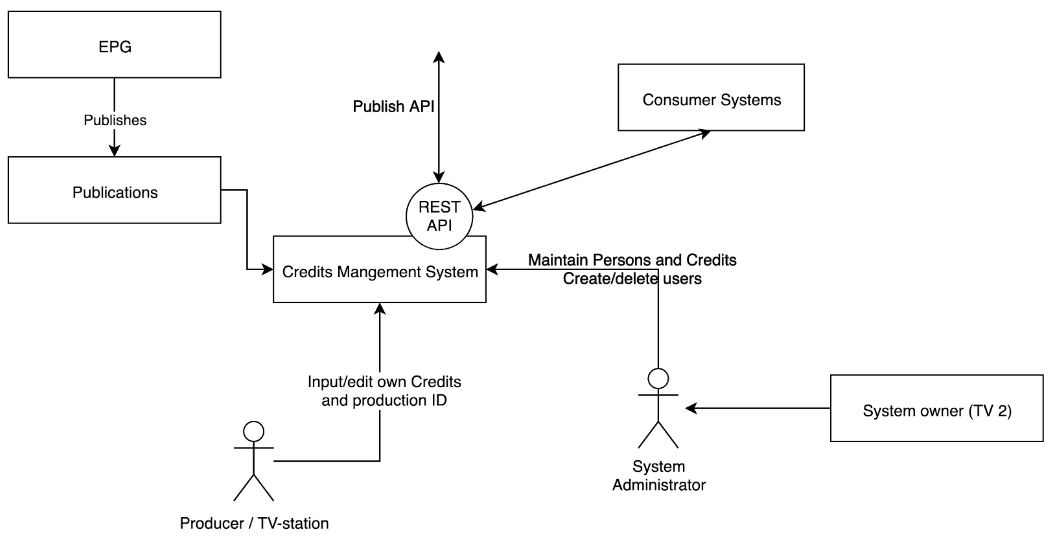
\includegraphics[scale=0.4]{figures/tv2_system.png}
    \caption{Foreslag til systemtegning - © TV2}
    \label{fig:tv2_system}
\end{figure}

\noindent % Det vi vælger fra:
I et produktionsklart system vil det være ideelt at have en webside, men dette har vi konkluderet som værende uden for projektet.